\newcommand{\authorinfotitle}{Vanessa Closius, Jonas Tietz, Tronje Krabbe}
\newcommand{\authorinfo}{Vanessa Closius, Jonas Tietz, Tronje Krabbe}
\newcommand{\titleinfo}{MMS}
\newcommand{\qed}{\square}

\documentclass[a4paper,11pt]{article}
%\usepackage[german,ngerman]{babel}
\usepackage[utf8]{inputenc}
\usepackage[T1]{fontenc}
\usepackage{lmodern}
\usepackage{amssymb}
\usepackage{mathtools}
\usepackage{amsmath}
\usepackage{enumerate}
\usepackage{breqn}
\usepackage{fancyhdr}
\usepackage{multicol}
\usepackage{tikz}
\usepackage{trfsigns}
\usepackage{float}

\author{\authorinfotitle}
\title{\titleinfo}
\date{\today}

\pagestyle{fancy}
\fancyhf{}
\fancyhead[R]{\authorinfo}
\fancyhead[L]{MMS Hausaufgaben}
\fancyfoot[C]{\thepage}
\allowdisplaybreaks
\begin{document}
	\maketitle
	\begin{enumerate}
		% Aufgabe 1
		\item[\textbf{1.}]
			If we simply pick one of the three shells at random, there
			is a one in three chance that we have picked the correct
			shell:
			\begin{align*}
				P = \frac{1}{3}
			\end{align*}
			However, if the thimblerigger uncovers a shell which does
			not hide the ball first, and allows us to switch, things
			change. This is an example of the Monty Hall Problem\footnote{https://en.wikipedia.org/wiki/Monty_Hall_problem}
			Intuitively, we would say that there is now a $50\%$ chance that
			our choice was the correct shell, and that our overall odds have
			not changed --- why would the thimblerigger revealing a loosing
			shell, which we have not even picked, alter our odds?
			However, we can actually increase our odds by switching
			our choice of shells to the remaining shell.
			See Table~\ref{table_monty_hall} for a concrete example
			of why switching is smart. The table shows all possible
			results, and assumes that we always pick Shell 1.

			\begin{table}[H]
			\centering
			\caption{Monty Hall Paradox}
			\begin{tabular}{| c | c | c | c | c |}
				\hline
				\textbf{Shell 1} & \textbf{Shell 2} & \textbf{Shell 3} & \textbf{Result if not switching} & \textbf{Result if switching} \\
				\hline
				nil & nil & \textbf{ball} & loose & \textbf{win} \\
				nil & \textbf{ball} & nil & loose & \textbf{win} \\
				\textbf{ball} & nil & nil & \textbf{win} & loose \\
				\hline
			\end{tabular}
			\label{table_monty_hall}
			\end{table}

			We can see that our odds of winning remain as one in three
			if we never switch, but increase to two in three if we do
			switch. Thus:
			\begin{align*}
				P = \frac{2}{3}
			\end{align*}
		% Aufgabe 2
		\item[\textbf{2.}]
			Our Python implementation supports the claims we made in the previous
			section. Without switching, the relative frequency of winning is
			at about $\frac{1}{3}$. With switching, it rises to about $\frac{2}{3}$.
			The plot which our program generates, shown in Figure~\ref{python_plot},
			shows this as well.
			\begin{figure}
				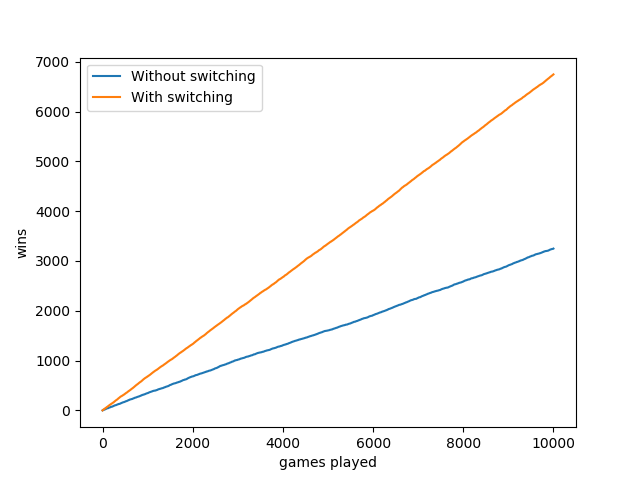
\includegraphics[scale=0.8]{relative_frequency_of_winning.png}
				\caption{The relative winning frequencies plotted by our software.}
				\label{python_plot}
			\end{figure}
	\end{enumerate}
\end{document}
